\documentclass[../Head/Main.tex]{subfiles}
\begin{document}
\begin{figure}[H]
\begin{subfigure}[b]{0.49\textwidth}
    \centering
    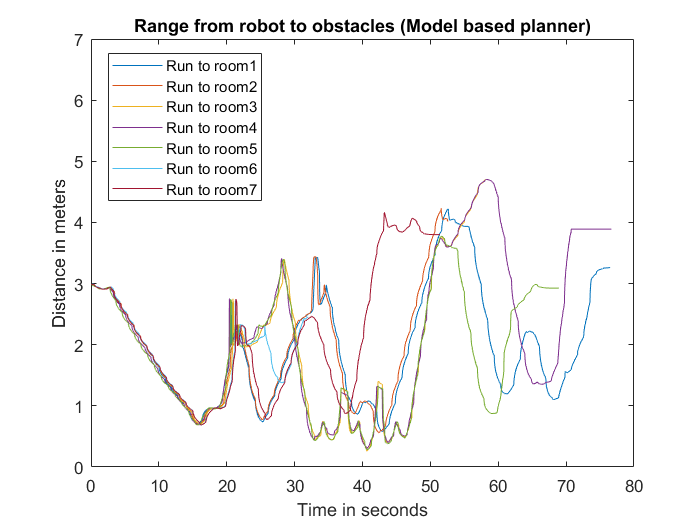
\includegraphics[width=0.95\textwidth]{PlotModelBasedObstacle}
    \caption{Illustration of the distance to the closest obstacle for room 1-7 for the model based planner}
    \label{fig:Model1}
  \end{subfigure}
  \hfill
  \begin{subfigure}[b]{0.49\textwidth}
    \centering
    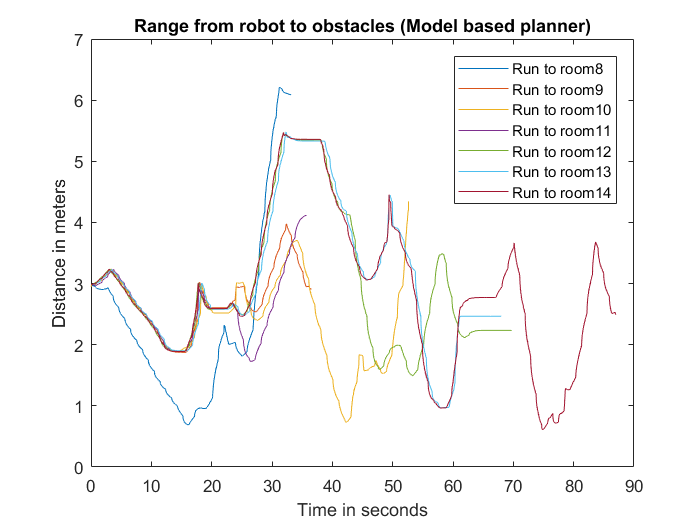
\includegraphics[width=0.95\textwidth]{Plot1ModelBasedObstacle}
    \caption{Illustration of the distance to the closest obstacle for room 8-14 for the model based planner}
    \label{fig:Model2}
  \end{subfigure}
  \hfill
  \begin{subfigure}[b]{0.99\textwidth}
    \centering
    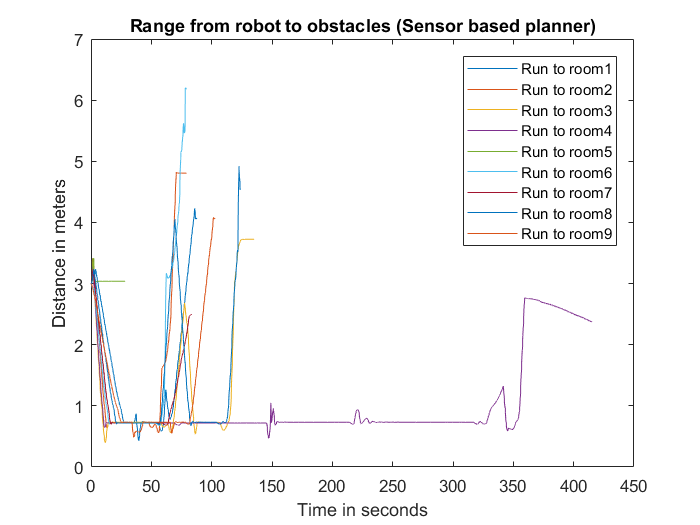
\includegraphics[width=0.47\textwidth]{PlotSensorBasedObstacle}
    \caption{Illustration of the distance to the closest obstacle for room 1-14 for the sensor based planner}
    \label{fig:Sensor 1}
  \end{subfigure}
  \caption{Illustration of the distance to the closest obstacle for room 1-14 for both planners}
\end{figure}
\end{document}